\begin{landscape}
\section{Anhang}
\subsection{Arbeitspakete und Aufwandschätzung}
\label{sub:arbeitspakete_und_aufwandschaetzung}
\begin{tabularx}{\linewidth}{|X|c|c|l|l|c|} \hline
\textbf{Arbeitspaket}&	\textbf{Aufwand Gesamt}&		\textbf{Verantwortlich}&	\textbf{Ausgeführt von}&	\textbf{Meilenstein}\\ \hline
UI-Design 																&	25h (6.5h pro Person)	&	Lion Kunz		&	Ganzes Team&	M1\\ \hline
Softwareentwurf															&	30h (7.5h pro Person)	&	Cyril Müller	&	Ganzes Team&	M1\\ \hline
DB-Design																&	5h	&	Sascha Bergmann	&	Cyril Müller&	M1\\ \hline
Java-Implementierung: Projekt und Grobstruktur, DB-Anbindung			&	10h	&	Lion Kunz		&	Sascha Bergmann&	M2\\ \hline
Grundgerüst Web erstellen												&	6h 	&	Cyril Müller	&	Dang Thien Nguyen&	M2\\ \hline
UI erstellen für Login, Logout, Registrierung, Benutzer bearbeiten		&	6h	&	Cyril Müller	&	Dang Thien Nguyen&	M2\\ \hline
UI erstellen für Datei hochladen, bearbeiten, anzeigen					&	8h	&	Lion Kunz		&	Dang Thien Nguyen&	M2\\ \hline
Java-Implementierung: Login, Logout, Zugriffskontrolle					&	8h	&	Dang Thien Nguyen&	Cyril Müller&	M2\\ \hline
Serverkonfiguration														&	3h	&	Sascha Bergmann	&	Cyril Müller&	M2\\ \hline
Java-Implementierung: Dateifunktionen, Zugriff beantragen, freigeben	&	12h	&	Dang Thien Nguyen&	Lion Kunz&	M2\\ \hline
\end{tabularx}
\clearpage
\begin{tabularx}{\linewidth}{|X|c|c|l|l|c|} \hline
\textbf{Arbeitspaket}&	\textbf{Aufwand Gesamt}&		\textbf{Verantwortlich}&	\textbf{Ausgeführt von}&	\textbf{Meilenstein}\\ \hline
UI erstellen für persönliche Startseite, Suchresultate					&	10h	&	Cyril Müller	&	Dang Thien Nguyen&	M3\\ \hline
UI erstellen für Modul und Gruppen bearbeiten, erstellen, anzeigen		&	9h	&	Sascha Bergmann	&	Lion Kunz&	M3\\ \hline
Java-Implementierung: Suche 											&	12h	&	Lion Kunz		&	Sascha Bergmann&	M3\\ \hline
Java-Implementierung: Modulfunktionen 									&	8h	&	Dang Thien Nguyen&	Cyril Müller&	M3\\ \hline
Java-Implementierung: Gruppe erstellen, bearbeiten, löschen 			&	8h	&	Lion Kunz		&	Cyril Müller&	M3\\ \hline
Java-Implementierung: Benutzer erstellen und bearbeiten 				&	8h	&	Cyril Müller	&	Lion Kunz&	M3\\ \hline
Test 																	&	30h (7.5h pro Person)	&	Dang Thien Nguyen&	Ganzes Team&	M4\\ \hline
Reserve 																&	22	&	Sascha Bergmann	&	&	M4\\ \hline
Dokumentation 															&	20h (5h pro Person)&	Lion Kunz		&	Ganzes Team&	M4\\ \hline
\textbf{Total}																	&	\textbf{240}	&		&	&	\\ \hline
\end{tabularx}
\end{landscape}


\subsection{Netzplan nach Abhängigkeiten}
\label{sec:netzplan_abhaengigkeiten}
\begin{figure}[H]
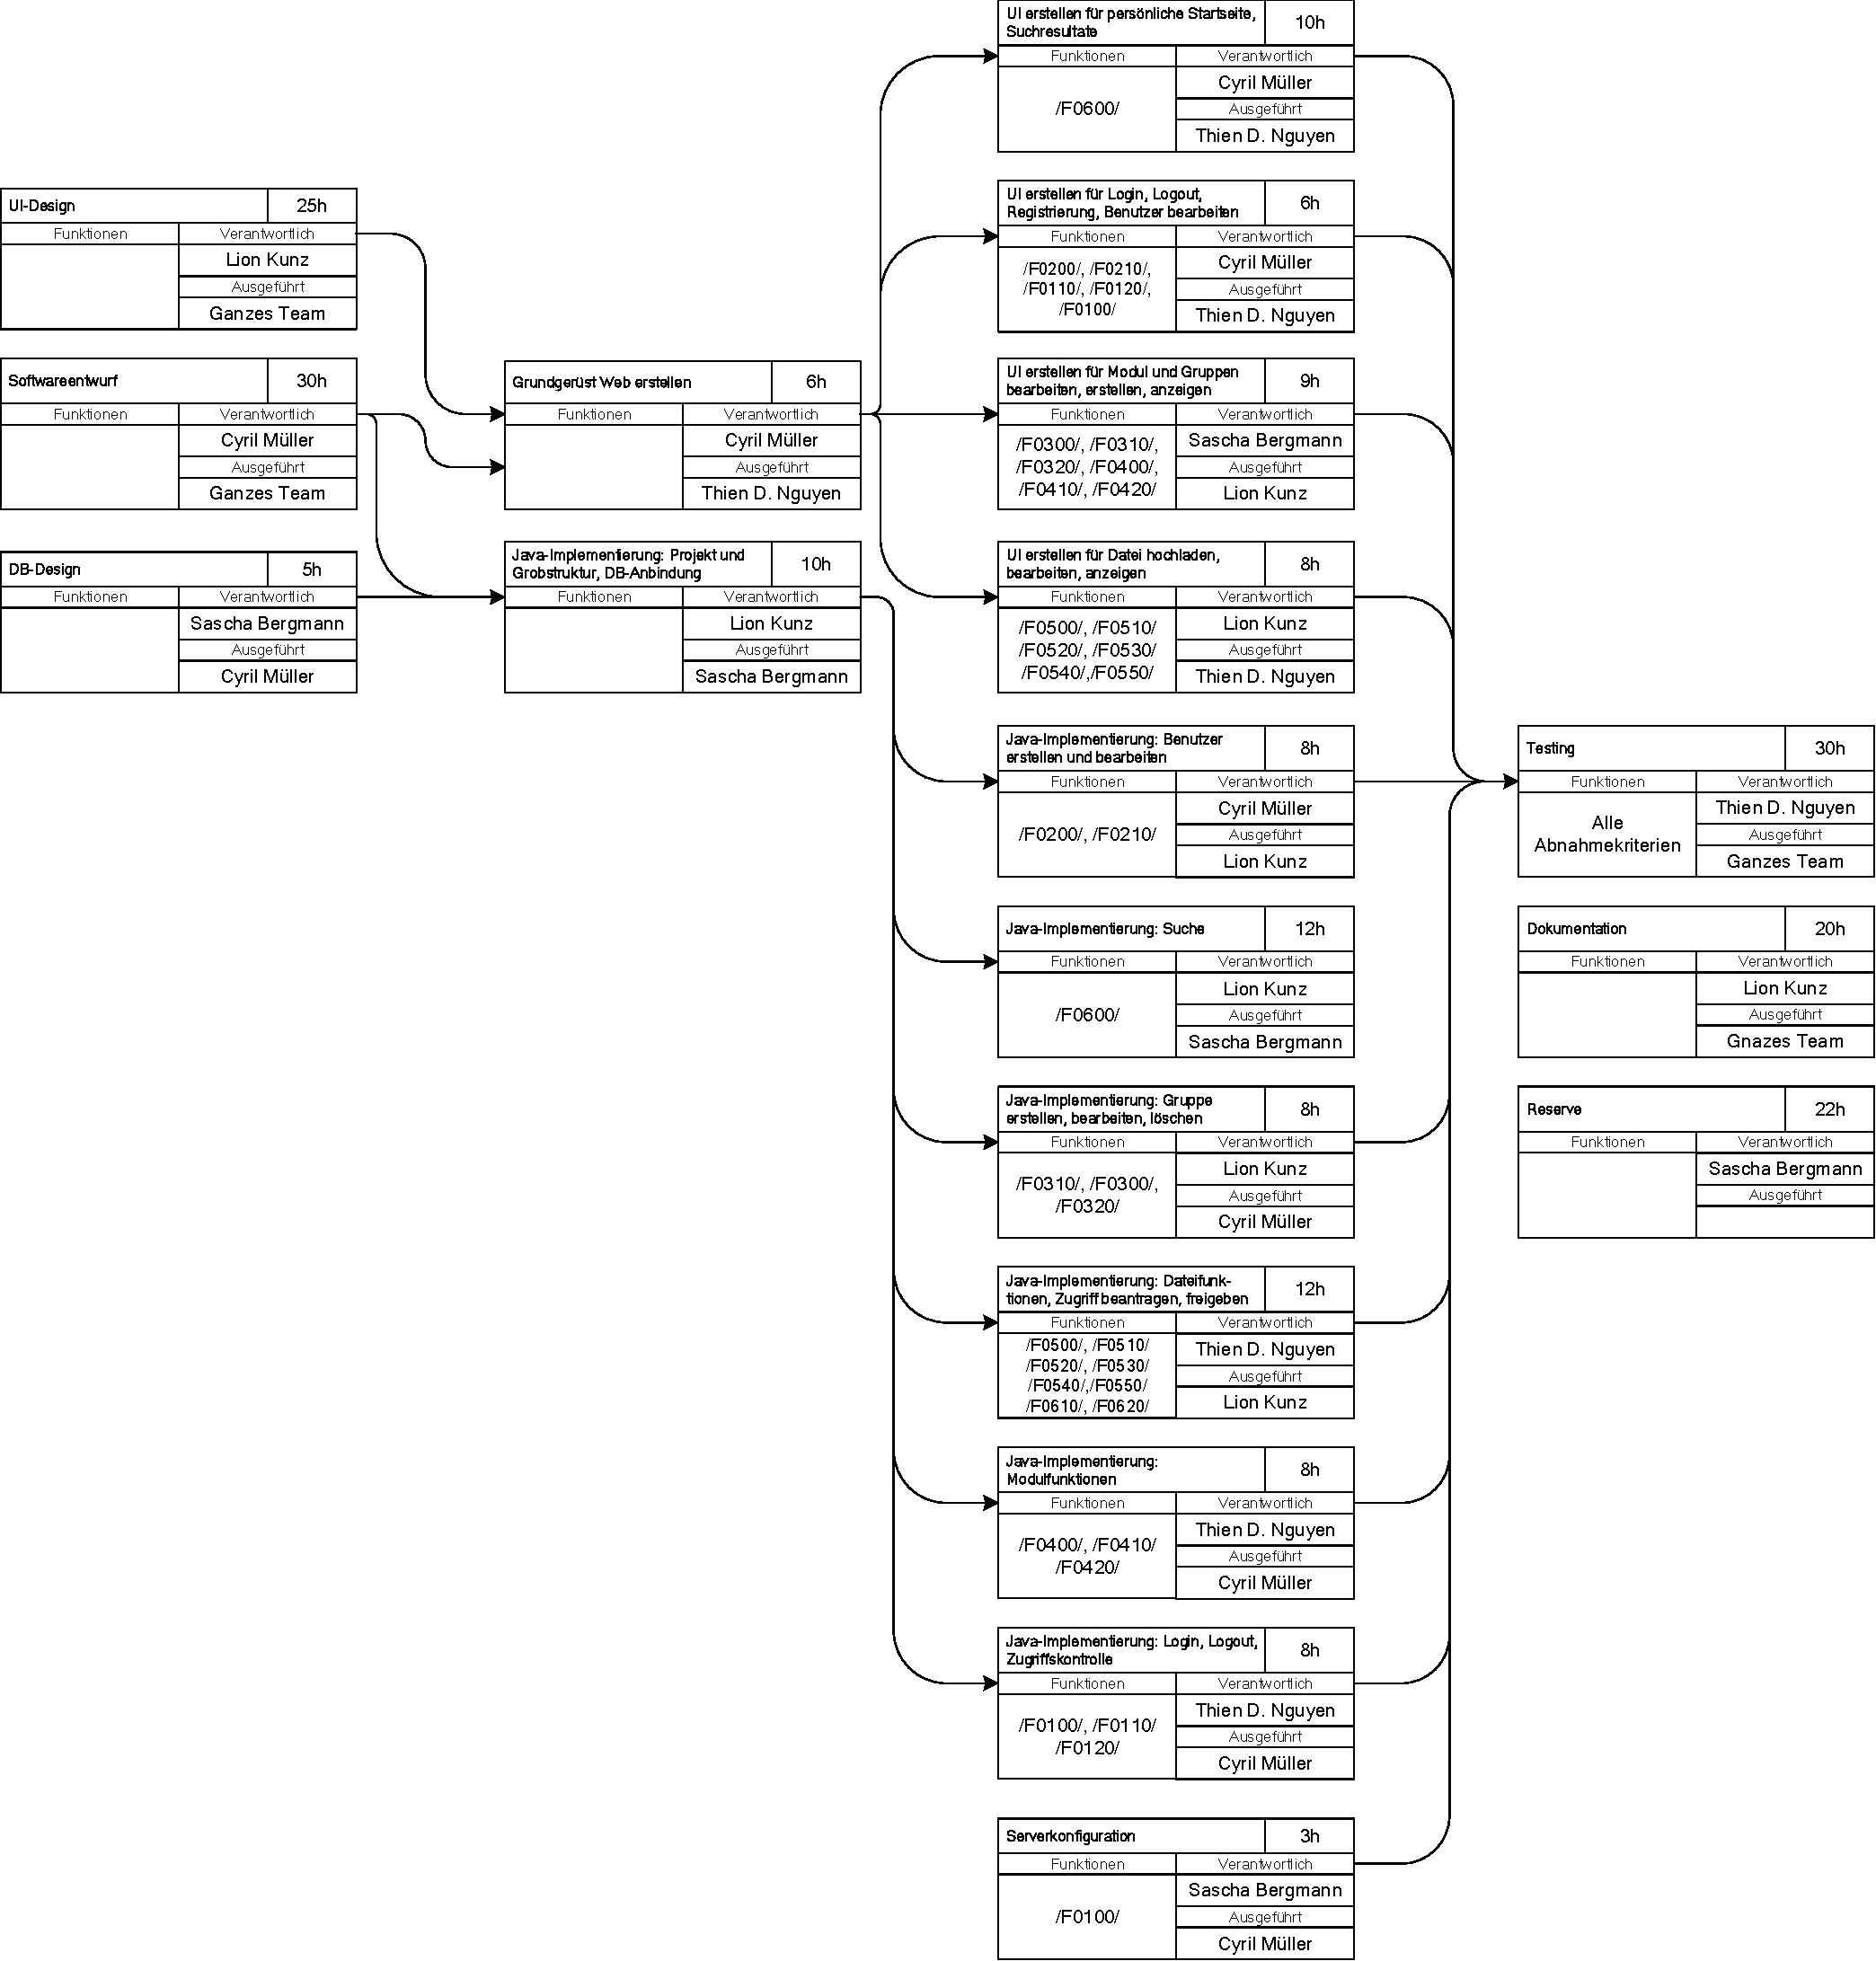
\includegraphics[width=1.1\linewidth]{graphics/netzplan_s1.pdf}
\caption{Darstellung des Netzplans, geordnet nach Abhängigkeiten der Arbeitspaketen.}
\end{figure}